\section{Simulation}%
\label{sec:simulation}
\emph{A python simulation has been created that will simulate the gas flow of the hydrogen power system, which provides insight to the behaviour of this complex system. This section describes the goal of the simulation, how it works and the results it produced.}

\subsection{Goal}
The goal of the SHARP-PS project is to develop a power system for a UAV that produces electricity from hydrogen using a fuel cell. This hydrogen will not be supplied by a hydrogen tank, but by a Cool Gas Generator (CGG) which will be developed by Solid Flow.

This system is quite complex and has many open variables that all influence each other.
For example, both the hydrogen generation and consumption rate affect the pressure of the hydrogen supply system. The hydrogen consumption rate is in turn affected by the frequency and length of purge events and the power demand on the fuel cell. The hydrogen production rate is dependent on the size of the CGG, but the size of the CGG also influences the volume available for the hydrogen thus also affecting the pressure in a different way.

In order to grasp this complex system of variables, a python simulation has been created that simulates the gas flows of the entire system. This allows the effect of changing each variable to be observed, which will be a useful tool during the development of the system.

\subsection{Process}
The core of the simulation are a set of volumes that contain either hydrogen or electricity, and several processes that move content from one volume to another at a rate determined by the system properties. Figure~\ref{fig:sim diagram} provides an overview of these volumes and processes, and the parameters each depends on.

\newcommand{\pytable}[2]{
    \begin{tabular}{c}
        \textbf{#1} \\
        \midrule
        #2          \\
    \end{tabular}
}

\newcommand{\cggstorage}{
    \pytable{CGG Storage}{Capacity \\ Amount}
}

\newcommand{\cggproc}{
    \pytable{CGG Production}{Rate}
}

\newcommand{\buffer}{
    \pytable{Buffer Volume}{Volume}
}

\newcommand{\fuelcell}{
    \pytable{Fuel Cell}{max power \\ min pressure \\ max pressure \\ normal massflow \\ purge massflow \\ purge duration \\ purge interval}
}

\newcommand{\control}{
    \pytable{Controller}{control scheme}
}

\newcommand{\battery}{
    \pytable{Battery}{Capacity}
}

\newcommand{\drone}{
    \pytable{Drone}{Climb Power\\ Cruise Power \\ Flight Profile}
}

\newcommand{\relief}{
    \pytable{Relief Valve}{Relief Pressure}
}

\begin{figure}[htp]
    \centering
    \scalebox{0.6}{
        \begin{tikzpicture}[node distance=37mm]
            \node (v_cgg) [pyvolume] {\cggstorage};
            \node (p_cgg) [pyprocess, right of=v_cgg] {\cggproc};
            \node (v_buffer) [pyvolume, right of=p_cgg] {\buffer};
            \node (p_fc) [pyprocess, right of=v_buffer] {\fuelcell};
            \node (p_control) [pyprocess, right of=p_fc] {\control};
            \node (v_battery) [pyvolume, right of=p_control] {\battery};
            \node (p_drone) [pyprocess, right of=v_battery] {\drone};

            \node (p_relief) [pyprocess, below of=v_buffer, yshift=17mm] {\relief};
            \node (v_relief) [pyvolume, below of=p_relief, yshift=2cm] {\textbf{Wasted H2}};

            \draw [arrow] (v_cgg) -- (p_cgg);
            \draw [arrow] (p_cgg) -- (v_buffer);
            \draw [arrow] (v_buffer) -- (p_fc);
            \draw [arrow] (p_fc) -- (p_control);
            \draw [arrow] (p_control) -- (v_battery);
            \draw [arrow] (v_battery) -- (p_drone);

            \draw [arrow] (v_buffer) -- (p_relief);
            \draw [arrow] (p_relief) -- (v_relief);

            \draw [arrow] (v_buffer) -- ++(0,3) -| ($(p_control.north) - (0.2,0)$);
            \draw [arrow] (v_battery) -- ++(0,3) -| ($(p_control.north) + (0.2,0)$);
        \end{tikzpicture}
    }
    \caption{Simulation Diagram}
    \label{fig:sim diagram}
\end{figure}

\subsection{Implementation}
The initial parameters chosen for the simulation are based on the mission scenario by Wren Aerospace. These parameters are listed in table~\ref{tab:direct_sim_parameters}. From these parameters, a preliminary fuel cell can be selected which will provide typical parameters for fuel cells in this range, visible in table~\ref{tab:derived_sim_parameters}. The final selecting of the fuel cell to be used will be discussed later in chapter~\ref{chap:design}. The simulation parameters may be adjusted at any time to suit the selected fuel cell.

\newcommand{\simpar}[3]{#1 & #2 & #3\\}

\begin{table}[htp]
    \centering
    \begin{subtable}[t]{0.3\textwidth}
        \centering
        \scalebox{0.85}{
            \begin{tabular}[t]{lrl}
                \toprule
                \textbf{Parameter} & \textbf{Value} & \textbf{Unit} \\
                \midrule
                \simpar{CGG Capacity}{160}{g}
                \simpar{Fuel Cell max Power}{200}{W}
                \simpar{Climb Power}{220}{W}
                \simpar{Cruise}{160}{W}
                \simpar{Flight time}{14}{h}
                \bottomrule
            \end{tabular}}
        \caption{Based on the Mission Scenario by Wren Aerospace}%
        \label{tab:direct_sim_parameters}%
    \end{subtable}%
    \hspace{\fill}
    \begin{subtable}[t]{0.3\textwidth}
        \centering
        \scalebox{0.85}{
            \begin{tabular}[t]{lrl}
                \toprule
                \textbf{Parameter} & \textbf{Value} & \textbf{Unit} \\
                \midrule
                \simpar{Min pressure}{0.35}{Bar}
                \simpar{Max pressure}{0.5}{Bar}
                \simpar{Normal massflow}{0.263}{g/min}
                \simpar{Purge massflow}{0.545}{g/min}
                \simpar{Purge duration}{1--2}{s}
                \simpar{Purge interval}{30--90}{s}
                % \simpar{CGG rate}{0.21}{g/min}
                \bottomrule
            \end{tabular}}%
        \caption{Derived from the selected Fuel Cell}%
        \label{tab:derived_sim_parameters}%
    \end{subtable}
    \hspace{\fill}
    \begin{subtable}[t]{0.3\textwidth}
        \centering
        % \flushright
        \scalebox{0.85}{
            \begin{tabular}[t]{lrl}
                \toprule
                \textbf{Parameter} & \textbf{Value} & \textbf{Unit} \\
                \midrule
                \simpar{CGG Amount}{1}{---}
                \simpar{CGG rate}{0.21}{g/min}
                \simpar{Buffer Volume}{0.1}{L}
                \simpar{Relief Pressure}{4}{Bar}
                \simpar{Battery Capacity}{500}{kJ}
                \bottomrule
            \end{tabular}}
        \caption{Chosen}%
        \label{tab:chosen_sim_parameters}%
    \end{subtable}%
    \caption{Simulation Parameters}%
    \label{tab:sim_parameters}%
\end{table}

% \emph{Something about control scheme and flight profile...}
The flight profile has not been determined yet, for the purposes of this simulation a climb of 1 hour has been chosen after which the drone will cruise for the rest of the mission.

The purpose of the controller is to limit the hydrogen consumption when the pressure in the buffer volume gets too low or when the battery is fully charged. For this purpose both an On---Off controller and a PID controller have been tested.

\subsection{Results}
Running the simulation with all parameters unchanged and as stated in the previous section produces the graph in figure~\ref{fig:sim default}. The pink line represents the power draw from the drone, this illustrates most clearly what phase of the mission is currently happening. Takeoff happens around half an hour into the simulation, then a 1 hour climb with high power demand after which the drone cruises for the rest of the mission, using less power. As a range was given for both climb and cruise power the simulation picks a random value in the range each timestep, hence this line appears very thick.

The red line represents the content of the battery. It starts empty and begins to charge, when it is at 50\% the drone starts liftoff. This uses more power than the fuel cell can provide, therefore the battery supplies the additional power and thus discharges over time. When the drone switches to cruising the battery can charge again slowly. Note how the battery discharges rapidly around the 14 hour mark. This is because the CGG has run out (indicated by the yellow line) and the fuel cell can no longer provide any power. At this point, all the power is delivered by the battery until it is at 10\%, then the mission is at an end or a new CGG is ignited in case multiple CGG's were brought on the mission.

\begin{figure}[htp]
    \centering
    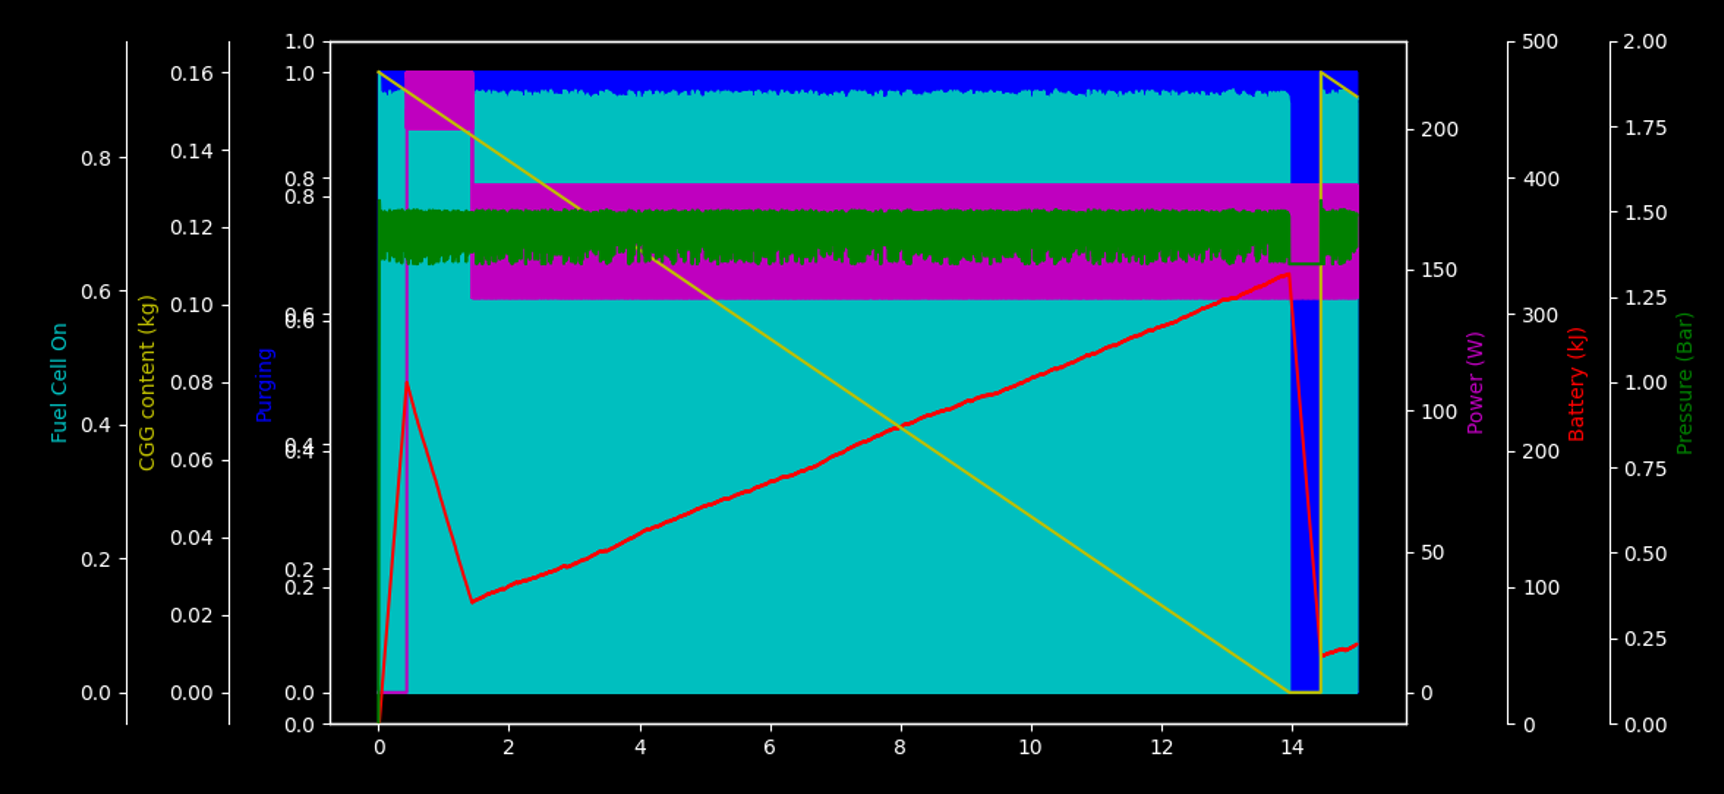
\includegraphics[width=\textwidth]{media/sim/default.png}
    \caption{Simulation Result}
    \label{fig:sim default}
\end{figure}

The green, blue and cyan lines indicate pressure in the buffer volume, whether a purge event is happening and how much power the fuel cell produces respectively. At the scale of figure~\ref{fig:sim default} their behaviour is poorly visible. Figure~\ref{fig:sim purge} provides a zoomed in view around the moment that a purge event is happening, there the behaviour of the three lines is better visible. Note however, that some lines have been excluded from this view and the scales have been altered for better visibility.

The blue line is at zero when no purge event is happening and jumps to one during a purge event. In the middle of the graph a purge event of around two seconds is visible. During the purge event the fuel cell uses hydrogen at an increased rate. Consequently, the pressure in the buffer volume drops to supply this extra hydrogen which can be seen in the green line. The controller notices this pressure drop and limits the power output of the fuel cell thereby limiting the hydrogen consumption, this can be seen by the cyan line dropping to zero.

After the purge event, the fuel cell is still limited, allowing the pressure in the buffer volume to build up again. When this pressure has been largely recovered, the fuel cell is allowed to produce power again. The reduction in power output from the fuel cell is compensated by the battery, which is visible in the red line.

\begin{figure}[htp]
    \centering
    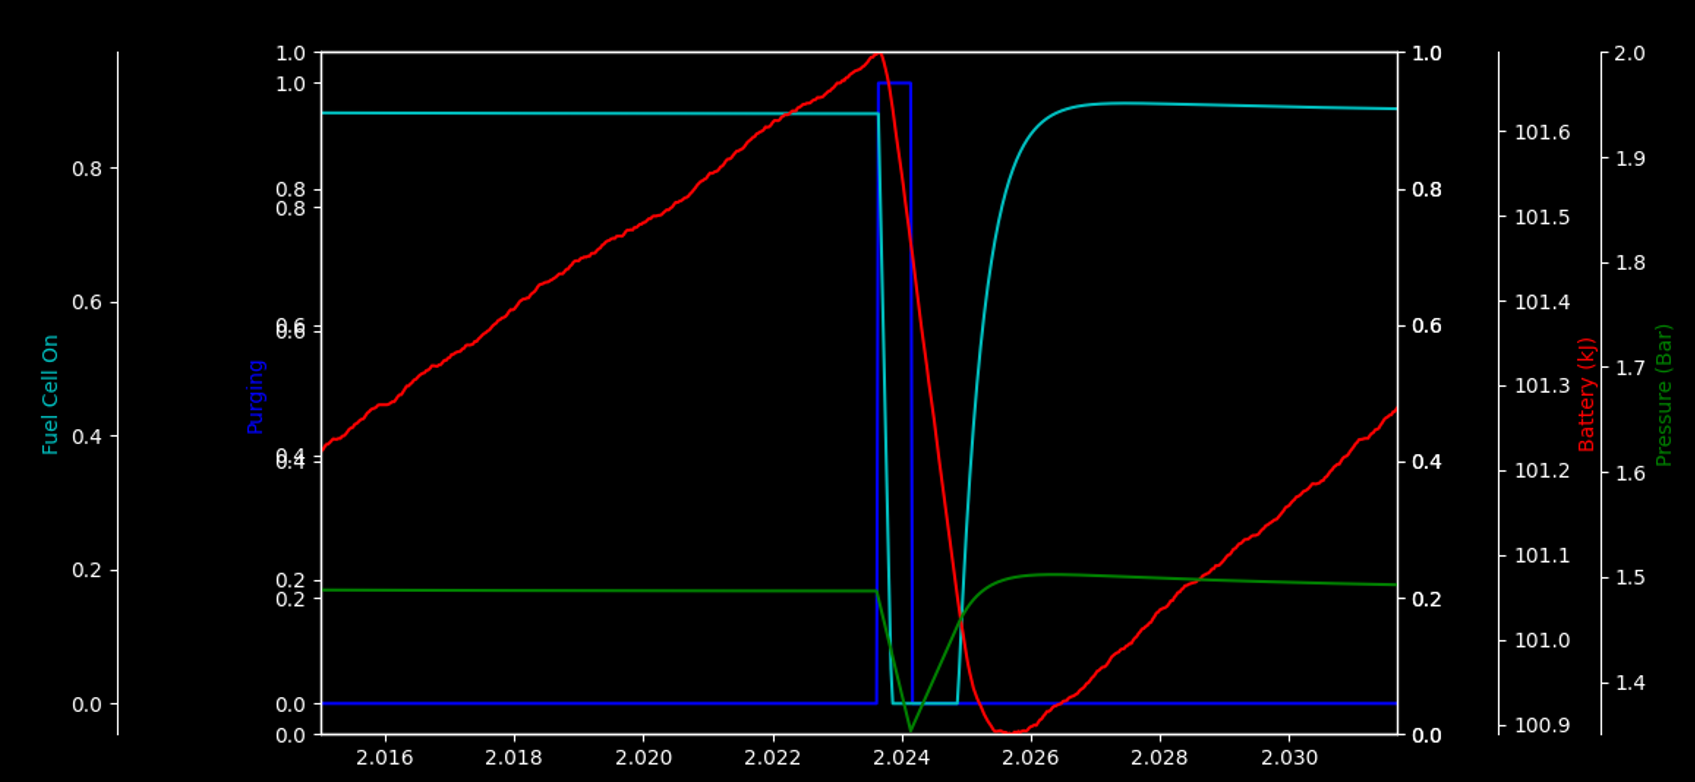
\includegraphics[width=\textwidth]{media/sim/purge.png}
    \caption{Purge Event}
    \label{fig:sim purge}
\end{figure}

\newpage
Many of the parameters used in this simulation were altered to investigate their effect on the overall system behaviour. These results were used during the design of the hydrogen power system, and as such will be discussed further in chapter~\ref{chap:design}.

The simulation results will also need to be verified against real-world test results. For this and other purposes a compressed air system will be developed that will perform the gas flow of the hydrogen power system but with compressed air instead of hydrogen. This air-equivalent system will be discussed throughout the following chapters. Its results will be compared with the results of this simulation in chapter~\ref{chap:testing}.
